

%!TEX root = /Users/daniel/Documents/thesis/thesis.tex
\chapter{Erkennung handgeschriebener Symbole} 

% (fold)
\label{cha:erkennung_handgeschriebener_symbole}

Die Erkennung handgeschriebener Symbole ist das Herzstück von Detexify. Hier wird einer unbekannten Eingabe von Daten ein \LaTeX-Symbol zugeordnet.
% Genau genommen wird der Eingabe eine Rangfolge von Symbolen zugeordnet, welche in der in \ref{sub:symbolsuche} beschriebenen Liste auftaucht, nachdem ein Nutzer ein Symbol gezeichnet hat.

Im Zentrum jeder Mustererkennungsaufgabe steht dabei der Erkennungsalgorithmus (\ref{sec:klassifizierung}). Je nach verwendetem Verfahren geht dem eine Vorverarbeitung (\ref{sec:vorverarbeitung}) und Merkmalsextraktion (\ref{sec:merkmale}) voraus. In diesem Kapitel beschreibe ich welche Verfahren bei Detexify zum Einsatz kommen und begründe die Auswahl.

\section{Terminologie} 

% (fold)
\label{sec:terminologie}

Wie in jedem Forschungsgebiet hat sich auch bei der Handschrifterkennung eine Nomenklatur entwickelt, die die verschiedenen Aspekte des Themas beschreibt.

Man unterscheidet zwischen \emph{Online}- und \emph{Offline}-Systemen \cite{Tappert:1990p10302}. Bei Online-Systemen wird die Erkennung durchgeführt während der Nutzer schreibt. Die Striche werden dabei vom Eingabegerät (häufig ein Grafiktablett, in Detexify i.d.R. eine Computermaus) als Funktion \( t \mapsto \alpha \), wobei \( \alpha \) den Zustand der Stiftspitze kodiert, an das System übertragen. Das heißt, es stehen für die Erkennung alle dynamischen Eigenschaften des Geschriebenen zur Verfügung, wie die Anzahl, Reihenfolge und Richtung der einzelnen Pinselstriche. Im Gegensatz dazu verarbeiten Offline-Systeme Scans von Geschriebenem, arbeiten also zu einem Zeitpunkt, wenn der Schreibvorgang längst beendet ist. Sie können also außer Pixeln keine weiteren Informationen verwenden. Detexify ist ein Online-System.

Der Zustand der Stiftspitze besteht in Online-Systemen in der Regel aus den Koordinaten $(x,y)$, der Information, ob die Spitze das Tablett berührt, oft bezeichnet mit \emph{pen-up} bzw. \emph{pen-down} und in manchen Fällen auch aus der Neigung und dem Azimut.

Aus den Daten werden dann häufig Merkmale abgeleitet, sog. \emph{Features}. Man unterscheidet zwischen \emph{globalen} und \emph{lokalen} Features \cite{Tapia:2007p9160}. Lokale Features sind solche, die von einzelnen Punkten auf einem Strich und dessen benachbarten Punkten abgeleitet werden. Globale Features werden hingegen von der Menge der Striche als Ganzes abgeleitet.

\TODO Typ 1,2,3 Klassifizierer

\section[Herausforderungen]{Herausforderungen der Erkennung von \LaTeX-Symbolen} Die Erkennung von handgemalten \LaTeX-Symbolen ist allein durch die enorme Anzahl der Symbole eine große Herausforderung \cite{Koerich:2003p1562}. Hinzu kommt, dass die Symbole aus sehr unterschiedlichen Alphabeten kommen. Es kommen lateinische, griechische, mathematische und weitere Symbole vor. Im Gegensatz zu asiatischen Sprachen, die ebenfalls sehr große Alphabete aufweisen\footnote{In Japan werden heute 6000-7000 Buchstaben verwendet. In China ist die Anzahl der im täglichen Leben verwendeten Buchstaben bei etwa 5000 \cite{Jaeger:2003p1097}}, ist jedoch die Anzahl und Reihenfolge der Striche nicht vorgegeben, was die Erkennung zusätzlich verkompliziert \cite{Watt:2005p1816}. Außerdem gibt es sehr viele sehr ähnliche Symbole wie $\rightarrow,\mapsto,\leadsto,\rightharpoonup,\hookrightarrow,\rightarrowtail$. Dazu kommen noch die Probleme vor der jede Handschrifterkennung steht, wie unterschiedliche Schreibstile sowohl von unterschiedlichen Schreibern als auch natürliche Variationen in der Schreibweise eines Einzelnen.

In Detexify wird diese Variation noch zusätzlich erhöht, da in den meisten Fällen eine herkömmliche Computermaus zum zeichnen der Symbole Verwendung findet, statt ein Grafiktablett, das eine gewohnte Stiftführung ermöglicht.

Ein guter Klassifizierer muss also einiges leisten um der Situation gerecht zu werden.

\section{Eingabe} \label{sec:input}

Die Eingabe erfolgt für Handschrifterkennungssysteme häufig durch ein Grafiktablett. Dies ist auch in Detexify eine Möglichkeit, aber nicht die Regel. Die in \ref{sub:symbolsuche} beschriebene Zeichenfläche erlaubt sowohl die Eingabe über ein Grafiktablett als auch per Maus, wobei letzteres jeder Computeranwender zuhause hat. Die Eingabe erfolgt in der Webanwendung und die Daten, die an Server gesendet werden und damit den Erkennungsalgorithmus erreichen sind durch das \ac{REST}-Interface (siehe \ref{subsub:erkennung}) spezifiziert. Die Daten bestehen aus einer Liste von Strichen, wobei jeder Strich aus einzelnen Punkten, die die Bewegung der Stiftspitze beschreiben, besteht. Ein Punkt beinhaltet seine Koordinaten $x$ und $y$ sowie einen Zeitstempel $t$. Im \ac{JSON}-Format sieht das wiefolgt aus:

\lstinline![[{"x":125.5, "y":219.133331298828, "t":1269620535913}, ...], [...]]!

\section{Vorverarbeitung und Normalisierung} 

% (fold)
\label{sec:vorverarbeitung}

Eine Vorverarbeitung (Preprocessing) der Daten bevor sie an die Erkennungsalgorithmen ausgeliefert werden, ist eine wirksame Methode um Rauschen, das z.B. durch Ungenauigkeiten der Eingabegeräte oder Unachtsamkeit des Schreibers, entstehen kann, zu relativieren. Vorverarbeitung kann aber auch überflüssige Informationen entfernen, die vom verwendeten Erkennungsalgorithmus nicht verwendet werden. Zudem kann durch Normalisierung der Daten ungewollte Variation reduziert werden. Es gibt kaum ein System zu Handschrifterkennung, das keine Vorverarbeitung durchführt \cite{Jaeger:2003p1097,Plamondon:2000p10303,Tappert:1990p10302}.

Die Auswahl der Maßnahmen hängt natürlich auch vom verwendeten Erkennungsalgorithmus ab. Detexify verwendet zur Klassifizierung \ac{DTW}, daher werden die folgenden Maßnahmen ergriffen:

\TODO Andere blasen sich hier mächtig auf und beschrieben alles haarklein mit vorher/nacher Schaubildern. Will ich das auch?

\begin{description}
  \item[Normalisierung der Größe und Position] Die ankommenden Striche werden verschoben und skaliert, so dass sie unter Beibehaltung ihres Seitenverhältnisses zentriert und maximal im Quadrat \([0,1]\times[0,1]\) liegen. Das ist notwendig, damit \ac{DTW} sinnvoll angewandt werden kann.
  \item[Entfernung von Haken]
  \TODO An den Enden von Strichen kann es zu Haken kommen, die beim Aufsetzen\dots
  \item[Glättung] Jeder Punkt eines Striches wird durch das arithmetische Mittel des Punktes und seiner beiden Nachbarn ersetzt. 
  \item[Äquidistante Verteilung] Da die Zeichenfläche im Browser in Detexify eine gewisse Abtastrate hat, die erstens Herstellerabhängig sein kann, und zweitens zeitabhängig ist, kann die Verteilung der Punkte auf den Strichen sehr ungleich sein. Daher werden die Punkte neu verteilt, so dass sie Entfernung zwischen zwei je Punkten gleichmäßig groß ist. Die Anfangs- und Endpunkte von Strichen werden dabei erhalten. 
  % \item[Verkettung] Da \ac{DTW} zwei Zeitreihen vergleicht, werden die Striche miteinander verkettet, so dass das Abstandsmaß direkt angewendet werden kann. \TODO das ist doch Mist! Das muss ich begründen. Verschlechtert ja die Erkennung total. Aber: Stroke joining macht manchmal Sinn... wenn Ende und Anfang nah beieinander liegen...
  \item[Richtungskorrektur der Striche] \TODO mache ich noch gar nicht. Sollte ich aber vielleicht. So wie bei \citet{Xie:2007p11427} z.B.
  \item[Sortierung der Striche] \TODO mache ich noch gar nicht. Sollte ich aber vielleicht. . So wie bei \citet{Xie:2007p11427} z.B.
\end{description}

% section preprocessing_und_normalisierung (end)
\section{Merkmale} \label{sec:merkmale}

\TODO das in Detexify verwendete Verfahren erfordert keine Merkmalsextraktion.
\citet{Xie:2007p11427} sagt man wisse noch nicht recht welche Merkmale für Handschrifterkennung optimal seinen.


\section{Klassifizierung} 

% (fold)
\label{sec:klassifizierung}

Die Klassifizierung ist in der Mustererkennung der Vorgang unbekannten Daten eine Klasse zuzuordnen. Im Fall von Detexify ist dies ein \LaTeX-Symbol. Sie kann auf unterschiedliche Weisen erfolgen.

Zur Erkennung einzelner handgeschriebener Symbole wurden bereits unterschiedlichste Klassifikationsverfahren verwendet \cite{Plamondon:2000p10303}. Um ein leistungsstarkes Backend für Detexify zu entwickeln musste also ein Verfahren ausgewählt und gegebenenfalls optimiert werden, dass den spezifischen Anforderungen der Anwendung und der Architektur gerecht wurde.

Die Anforderungen sind die folgenden:
\begin{description}
  \label{desc:anforderungen} 
  \item[Adaptionsfähigkeit] Es sollte jeder Zeit ein Training zusätzlicher Symbole möglich sein. 
  \item[Skalierbarkeit] Die Erkennungsraten sollten auch bei einer großen Anzahl von Klassen gut sein. 
  \item[Laufzeitverhalten] Das Laufzeitverhalten sollte eine Erkennung in Echtzeit ermöglichen. 
  \item[Interaktivität] Es sollten die besten $N$ Symbole zur Auswahl angezeigt werden. 
\end{description}

Ein besonderes Interesse galt in meinem Fall natürlichen den Verfahren, die für Symbolerkennung, insbesondere mathematischer Symbole, bereits erfolgreich eingesetzt wurden. Dabei handelt es sich um \ac{SVM}, \ac{HMM} und \ac{DTW}. Es gibt auch einige wenige Strukturelle Ansätze.

\subsection{Strukturelle Methoden} \label{sub:strukturelle_methoden}

Strukturelle Methoden basieren auf der Annahme, dass Handschrift aus elementaren Formen, auch Allographen genannt, besteht. Die Darstellung einer Klasse erfolgt dann als strukturelle Repräsentation (z.B. als Baum oder Graph) bestehend aus diesen Allomorphen. Die Vorgehensweise lässt sich am besten an einem Beispiel illustrieren. \citet{Fitzgerald:2004p10858} stellen mathematische Symbole als eine Kombination von Merkmalen der Typen \emph{Linie}, \emph{C-Form} oder \emph{O-Form} dar. Diese Merkmale werden mithilfe von Fuzzylogik aus den Strichen extrahiert und zur Zuordnung des richtigen Labels kommt wieder Fuzzylogik zum Einsatz. Dabei haben sie für jede Symbolklasse, die sie verwenden eine eigene Fuzzy-Regel erstellt. Im zitierten Artikel waren das Regeln für die Zahlen 1-9 und kleingeschriebene lateinische Buchstaben. Es ist offensichtlich, dass ein solches Vorgehen für Detexify mit nahezu 1000 Symbolklassen nicht in Frage kommen kann. Zum Problem für jede Klasse ein Modell zu definieren kommt hinzu, dass das System nicht \emph{adaptionsfähig} im in \ref{desc:anforderungen} definierten Sinne ist, da jedes neue Symbol ein neues Modell braucht. Ohnehin ist es schwierig bei einer so großen Anzahl von Symbolklassen eine gemeinsame Struktur zu finden, die einen Strukturellen Ansatz praktikabel macht. Aus den genannten Gründen habe ich Strukturelle Methoden als ungeeignet für Detexify verworfen.

\subsection{Künstliche Neuronale Netze} \label{sub:kuenstliche_neuronale_netze}

Neuronale Netze haben bekanntlich Schwierigkeiten, wenn die Anzahl der Klassen groß ist \cite{Jaeger:2003p1097}. Dementsprechend ist die Anzahl der in Übersichtsartikeln zur Erknennung von Mathematischen Formeln wie \cite{Chan:2000p559} und \cite{Tapia:2007p9160} zitierten Arbeiten, die neuronale Netze verwenden, äußerst gering und ich habe keinen nach 1996 veröffentlichten Artikel gefunden, der Neuronale Netze für diese Aufgabe verwendet. Neuronale Netze können also als irrelevant abgehakt werden.

\subsection[SVM]{SVM - Support Vector Machines} \label{sub:svm}

\ac{SVM}s haben sich zu einem beliebten Klassifikationsverfahren für bestimmte Problemklassen entwickelt. Bei dem Verfahren betrachtet man eine Menge von (Trainings-)Objekten in einem Verktorraum (dem Merkmalsraum). Jedes Objekt gehört einer Klasse an und nun legt man eine Hyperebene so durch den Raum, dass die Klassen getrennt und der Rand zu beiden Seiten der Hyperebene maximal wird. Das Verfahren ist natürlich nur sinnvoll, wenn sich die Klassen linear trennen lassen. Ist dies nicht der Fall, kann man sich des Kernel-Tricks bedienen und den Merkmalsraum auf einen höherdimensionalen Verktorraum abbilden, in dem die Klassen linear trennbar sind.

\ac{SVM}s sind binäre Klassifizierer. Um sie also bei $N>2$ Klassen verwenden zu können gibt es unterschiedliche Strategien. Zum einen gibt es die \ac{WTA}-Strategie bei der $N$ binäre Klassifizierer konstruiert werden, wobei der $i$-te Klassifizierer $\rho_i$ die Klasse $C_i$ und $C_i^{\complement}$ (also alle anderen Klassen) unterscheidet. Einem unbekannten Objekt $x$ wird dann die Klasse zugeordnet, deren SVM $\rho_i$ das beste Ergebnis zurückliefert\footnote{Eine SVM ist als Funktion realisiert, die die Lage eines Eingabevektors zur Hyperebene zurückgibt. Das Ergebnis ist besser wenn der Eingabevektor weit auf der richtigen Seite liegt, also der Abstand zur Ebene größer ist.}. Zum anderen gibt es die \ac{MWV}-Strategie bei der für jedes Paar von Klassen $C_i$ und $C_j$ ein Klassifizierer $\rho_{ij}$ mit den Objekten aus $C_i$ gegen die Objekte aus $C_j$ trainiert wird. Für ein unbekanntes Objekt $x$ werden nun alle $N(N-1)/2$ Klassifizierer nach ihrer Stimme gefragt und die Klasse mit den meisten Stimmen gewinnt. Weitere Kombinationsstrategien finden sich in \cite{Duan:2005p11426} und \cite{Platt:2000p11488}.

\TODO SVM in Literatur, insb. Kernel-Trick Bernhard Schölkopf, Alex Smola: Learning with Kernels: Support Vector Machines, Regularization, Optimization, and Beyond (Adaptive Computation and Machine Learning), MIT Press, Cambridge, MA, 2002, ISBN 0-262-19475-9. Ingo Steinwart, Andreas Christmann: Support Vector Machines, Springer, New York, 2008. ISBN 978-0-387-77241-7. 602 pp.

\citet{Tapia:2003p11202,Tapia:2005p11236} verwenden \ac{DAGSVM}s \cite{Platt:2000p11488} zur Symbolerkennung in einem System, dass u.a. mathematische Formeln auf einer Elektronischen Tafel erkennt.
\citet{Golubitsky:2009p2456,Keshari:2008p528,Golubitsky:2009p2321} stellen Mathematische Symbole als Merkmalsvektor bestehend aus der Koeffizienten einer Funktionalapproximation der Striche dar und trainieren damit \ac{SVM}s, die sie mit \ac{MWV} kombinieren. Die genannten Autoren berichten auch von guten Ergebnissen — jedoch hätten \ac{SVM}s für Detexify einen entscheidenden Nachteil.

Das Hauptproblem besteht darin, dass SVMs schlecht nachtrainiert werden können. Um nachträglich ein neues Trainingsmuster hinzuzufügen, müssen bei $N$ Klassen beim deutlich besseren MWV-Verfahren \cite{Duan:2005p11426} $N-1$ SVMs angepasst (das heißt die Hyperebenen neu ausgerechnet) werden. Um eine neue Klasse hinzuzufügen müssen ebenfalls $N$ neue SVMs eingefügt werden. Ein inkrementelles Training ist also bei SVMs gar nicht denkbar. SVMs sind also ebenfalls nicht \emph{adaptionsfähig} und kommen daher nicht wirklich in Frage.

\subsection[HMM]{HMM - Hidden Markov Models} \label{sub:hmm}

\ac{HMM} sind ein statistisches Mustererkennungsverfahren, das schon seit langem in der Spracherkennung eingesetzt wird \cite{Rabiner:1989p11574}. Das liegt daran, dass es besonders geeignet ist zeitliche Muster zu modellieren und außerdem Segmentierung und Klassifizierung integriert \cite{Kosmala:1998p11691}. Der Merkmalsvektor darf dabei von Muster zu Muster in der Länge variieren.
Dabei beschreibt ein HMM einen diskreten Markovprozess $q=(q_t)_{t=0,1.\dots}$ dessen Zustandsfolge aber nicht sichtbar (also verborgen, daher der Name) ist. Stattdessen sieht der Beobachter eine Symbolfolge $\mathbf{O}=O_1\dots O_T, O_t\in V$ aus einem endlichen Alphabet $V=\{v_i\}_{i=1\dots K}$ wobei zu jedem Zeitpunkt $t$ jeweils $O_t$ nur vom verborgenen Zustand $q_t$ der diskreten Markovkette abhängt. Abb.~\ref{fig:hmm} illustriert das Modell. Eine ausführliche Einführung zu HMMs inklusive Erklärung von diskreten Markovprozessen findet sich bei \citet{Rabiner:1989p11574}. 

\begin{figure}
  \centering 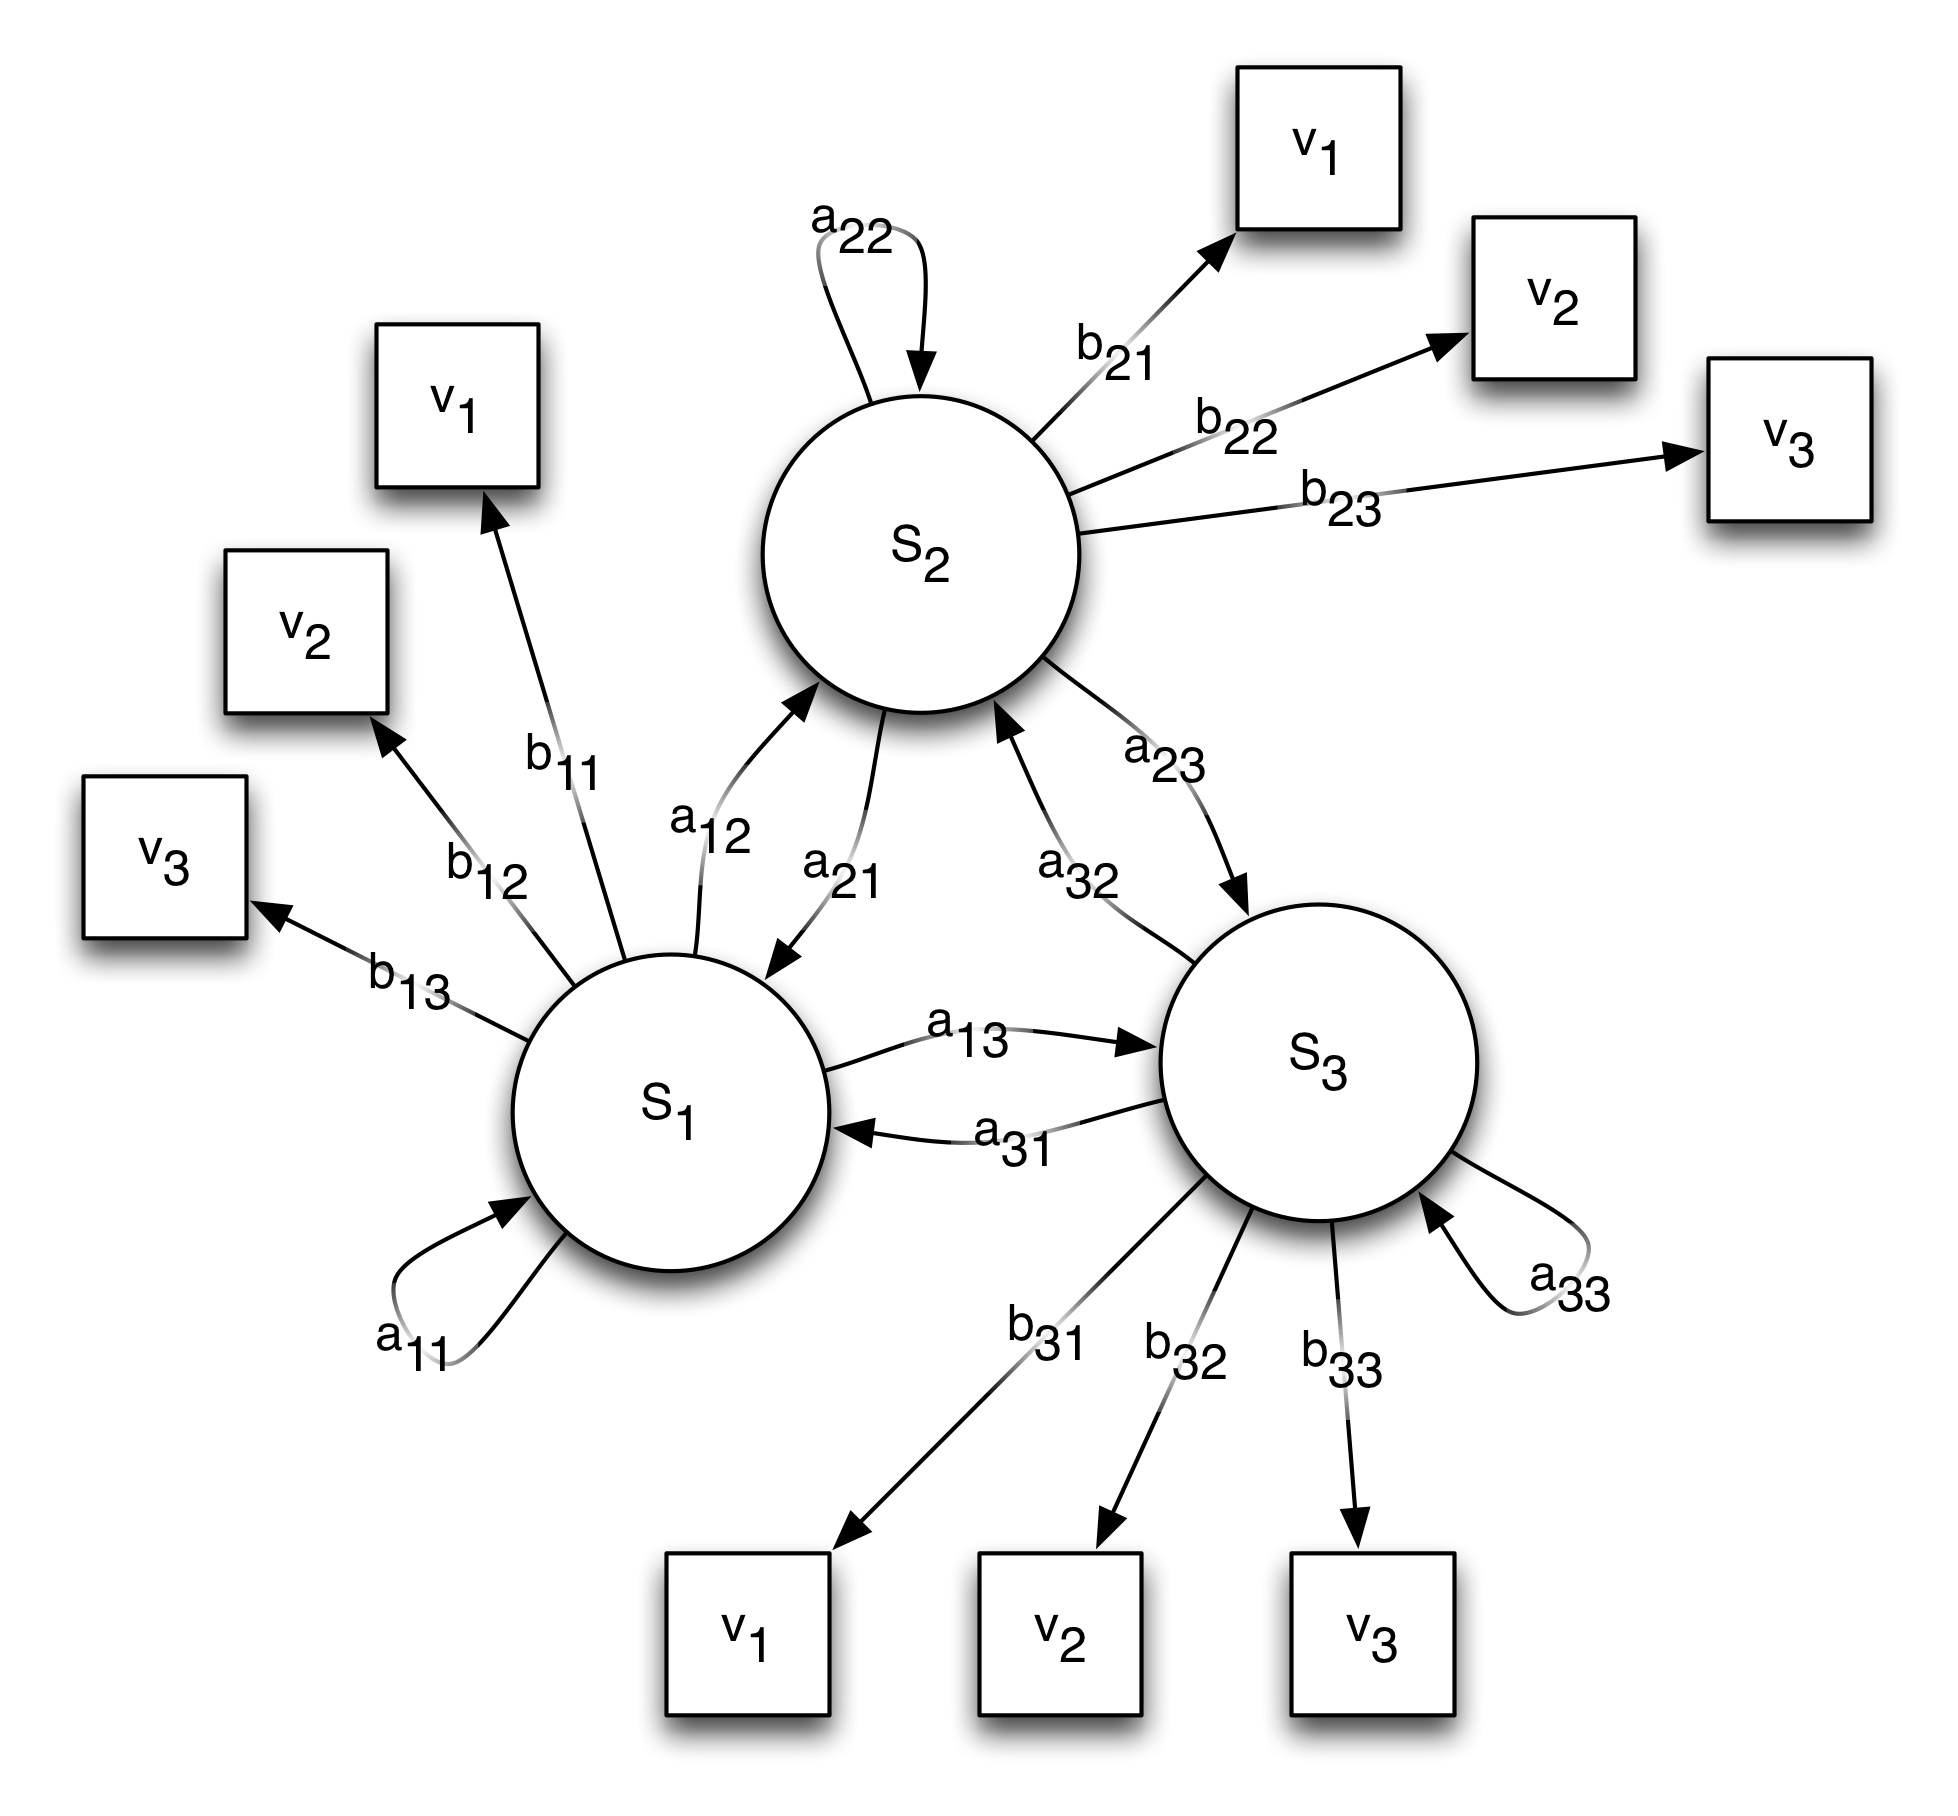
\includegraphics[width=\textwidth]{figures/hmm.png}
  \caption{HMM}
  \label{fig:hmm}
\end{figure}

Man verwendet eine HMM dann folgendermaßen: Jede Klasse $C_i$ bekommt eine HMM $\lambda_i$ deren Parameter anhand einer Stichprobe trainiert werden. Einem unbekannten Objekt, das als Folge $\mathbf{O}$ von Merkmalsvektoren beobachtet wird, wird dann die Klasse zugeordnet, für die die Wahrscheinlichkeit $P(\mathbf{O}|\lambda_i)$ (\TODO ich würde das $P_{\lambda_i}(\mathbf{O})$ schreiben...), dass die Folge von der zugehörigen HMM erzeugt wurde, maximiert wird.

\citet{Xie:2007p11427} beschreibt ein System zur Erkennung mathematischer Symbole, das auf HMM basiert. In derselben Arbeit wird auch ein Klassifizierer, der auf DTW basiert vorgestellt, und für diesen werden beeindruckende Erkennungsraten von im besten Fall 94.8 \% angeben. Obwohl sich ein Vergleich angeboten hätte werden jedoch für das HMM-basierte System keine absoluten Erkennungsraten vorgestellt, sondern lediglich relative Veränderungen, wenn mit den Parametern der HMM gespielt wird. Das stimmt etwas nachdenklich.

\citet{Winkler:1996p11716} kombiniert mehrere HMMs, die mit unterschiedlichen Merkmalen trainiert werden, und erreicht bei einem Alphabet von 84 Symbolen im besten Fall eine Erkennungsrate von 91 \%.

Von der Leistungsfähigkeit her scheinen HMMs also durchaus eine Option für Detexify zu sein. Ein Problem ergibt sich aber wieder bei der \emph{Adaptionsfähigkeit}: Die Effektivität eines HMM hängt von ihrer Modellierung ab (Anzahl der Zustände, Übergangswahrscheinlichkeiten, Ausgabewahrscheinlichkeiten) und diese müssten idealerweise für jede Symbolklasse individuell optimiert werden \cite{Fitzgerald:2005p331}. Das Hinzufügen einer neuen Symbolklasse umfasst also die Definition eines neuen HMMs und dessen Training.

\subsection{Nächste-Nachbarn-Klassifikation} \label{sub:knn}

Der $k$-nächste-Nachbarn-Algorithmus ist eines der einfachsten Verfahren um einem unbekannten Muster eine Klasse zuzuweisen. Dazu werden als Training einfach Vertreter der Klassen in einem Merkmalsraum gespeichert. Dem unbekannten Muster wird dann durch ein Mehrheitsvotum der $k$ nächsten Nachbarn eine Klasse zugeordnet. Eine zentrale Rolle nimmt dabei das Abstandsmaß, das die Nachbarschaft bestimmt, ein \cite{Jaeger:2003p1097}. Es beeinflusst die Güte der Klassifikation, aber auch durch seine Laufzeitkomplexität den zeitlichen Aufwand des Vorgangs. \TODO Literatur - Bücher?

Dabei ist KNN besonders bei Problemen beliebt, in denen die Anzahl an Klassen sehr hoch ist, wie beispielsweise bei japanischen Schriftzeichen \cite{Jaeger:2003p1097}. Eine Analyse zur Eignung für Detexify scheint also angebracht.
\TODO Laut Jiang Script Kapitel 4 ist KNN mit vielen Trainingsdaten nahezu so gut wie Bayes (optimal)
% \citet{Tappert:1990p10302} sagt bei Online-Erkennung reichen wegen der Interaktivität einfachere Methoden, was bei mir ja voll zutrifft.

Die Bedingung der \emph{Adaptionsfähigkeit}, die ich in \ref{sec:klassifizierung} gefordert hatte, die bei den bisher vorgestellten Verfahren schwierig umzusetzen war, ist dabei bei der Nächste-Nachbarn-Klassifikation auf natürliche Weise dadurch gegeben, dass neue Trainingsmuster einfach nur gespeichert werden müssen. \emph{Interaktivität} kann leicht realisiert werden, indem jeder Klasse ein auf dem Abstandsmaß basierender Wert zugewiesen wird. So erhält man für ein unbekanntes Muster eine Rangfolge der Klassen.

Es ist also zu klären, ob es ein Abstandsmaß gibt, das die Bedingungen \emph{Skalierbarkeit} und \emph{Laufzeitkomplexität} miteinander vereinen kann.

\subsection[DTW]{DTW - Dynamic time warping} \label{sub:dtw}

Ein vielversprechendes Abstandsmaß wurde bereits in \ref{sub:hmm} erwähnt. Es wird \emph{dynamic time warping} oder auch \emph{elastic matching} genannt. \citet{Xie:2007p11427} erreicht damit für die Erkennung mathematischer Symbole  eine Erkennungsrate von 94.8 \%. Auch \citet{Golubitsky:2009p2433} bemerken:
% In diesem Paper gibts auch Infos zum verwendete Datensatz. Weitere Statistiken zu Elastic matching Parametern.
\begin{quote}
  Among the distance measures used for classifying handwritten mathematical symbols, the elastic matching distance is known to be one of the most accurate.
\end{quote}

\citet{Golubitsky:2009p1842} vergleichen DTW mit einem eigenen Abstandsmaß, das zwar deutlich schneller zu berechnen ist, aber auch 1-1,5\% schlechtere Erkennungsraten liefert. \citet{Labahn:2008p10301} kombinieren DTW mit weiteren Methoden in einem System, das die handschriftliche Eingabe von Formeln in ein \ac{CAS} ermöglicht.
Auch \citet{Vuong:2010p10279} verwenden DTW % mit Steigung und Krümmung
zu Erkennung mathematischer Symbole in einer erst kürzlich veröffentlichten Arbeit zum Thema Web-basiertes CAS mit handschriftlicher Eingabe. Es ist auffällig, dass gerade aktuellere Arbeiten DTW einsetzen. Obwohl das Verfahren schon so lange bekannt ist \cite{Tappert:1982p10305}, ist es immer noch konkurrenzfähig.

Aus diesen Gründen ist die Wahl für die Klassifikation in Detexify auf DTW gefallen. Damit war die Aufgabe also den Algorithmus so zu implementieren und zu optimieren, dass die Bedingungen \emph{Skalierbarkeit} und \emph{Laufzeitkomplexität} erfüllt sind.

\section{DTW} % (fold)
\label{sec:dtw}

Im folgenden wird der klassische DTW-Algorithmus beschrieben und unterschiedliche Optimierungsmöglichkeiten werden diskutiert.

\subsection{Der klassische DTW-Algorithmus} % (fold)
\label{sub:der_klassische_dtw_algorithmus}

Seien zwei Folgen von Punkten
\begin{align}
  \label{eqn:a}
  A &= a_1, \dots, a_n \\
  \label{eqn:b}
  B &= b_1, \dots, b_m
\end{align}
in einem Raum \( S \ni a_i, b_i ~\forall~i \) und %die Menge von Abbildungen
% \begin{equation*}
%   \label{eqn:mappings}
%   F = \{f:\{1,\dots,n\} \rightarrow \{1,\dots,m\}, ~f~\text{surjektiv, monoton wachsend} \}  
% \end{equation*}
\( \delta : S\times S \rightarrow \mathbb{R}_0^+ \) eine Kostenfunktion
gegeben. In der Regel sind \(A\) und \(B\) Folgen in einem metrischen Raum z.B. \(\mathbb{R}^n\) und \(\delta\) ist eine Metrik.
Betrachten wir nun \( n\times m\)-Matrix 
\begin{equation} \label{eqn:matrix}
  M = (d_{i,j})_{i=1\dots n, j=1\dots m} ~\text{mit}~ d_{i,j} = \delta(a_i,b_j)
\end{equation}
, dann ist ein Warping-Pfad ein stetiger (im unten erläuterten Sinne) Pfad durch diese Matrix. 

\begin{align}
  W = w_0,\dots,w_K \hspace{1cm} w_l = (i,j)_l
\end{align}

$K$ ist dabei die Länge des Warping-Pfads. Die Stetigkeit des Pfads unterliegt den folgenden Bedingungen:

\begin{description}
  \item[Randbedingung] \( w_1 = (1,1) \) und \( w_K = (n,m) \). Dadurch beginnt der Warping-Pfad in der linken unteren Ecke der Matrix und endet in der rechten oberen Ecke.
  \item[Stetigkeitbedingung] Gegeben \( w_k = (i,j) \) und \( w_{k-1} = (i',j') \) so muss gelten \( i-i' \leqslant 1 \) und \( j-j' \leqslant 1 \). Dadurch sind nur Schritte zu benachbarten Zellen (auch diagonal) erlaubt.
  \item[Monotoniebedingung] Gegeben \( w_k = (i,j) \) und \( w_{k-1} = (i',j') \) so muss gelten \( i-i' \geqslant 0 \) und \( j-j' \geqslant 0 \). Dadurch werden rückwärtige Schritte (nach links oder unten) verhindert.
\end{description}

Es gibt natürlich einige Pfade die diese Bedingungen erfüllen. Nennen wir die Menge dieser Pfade
\[ \mathcal{W}=\{W~\text{ist Warping-Pfad}\} \]
dann ist der DTW-Abstand definiert durch
\begin{equation}
  \label{eqn:dtw}
  DTW(A,B) = \min_{W \in \mathcal{W}}{\frac{\sum_{i=1}^K d_{w_i}}{K}}
\end{equation}
. Dabei ist \( d_{w_i} \) das entsprechende Element der Matrix \ref{eqn:matrix}.

Diese abstrakte Definition bedeutet anschaulich, dass die Punkte in den zwei Folgen einander elastisch zugeordnet werden können, wobei es einige Beschränkungen gibt. Der erste Punkt der ersten Folge wird immer dem ersten Punkt der zweiten Folge und der letzte Punkt der ersten Folge immer dem letzten Punkt der zweiten Folge zugeordnet werden. Dazwischen müssen die Punkte zwar in der richtigen Reihenfolge bleiben und es dürfen keine übersprungen werden, aber es sind Mehrfachzuordnungen erlaubt. Gesucht wird die Zuordnung, die den Abstand minimiert. Abbildung~\ref{fig:dtw} illustriert dies.

\begin{figure}
  \centering 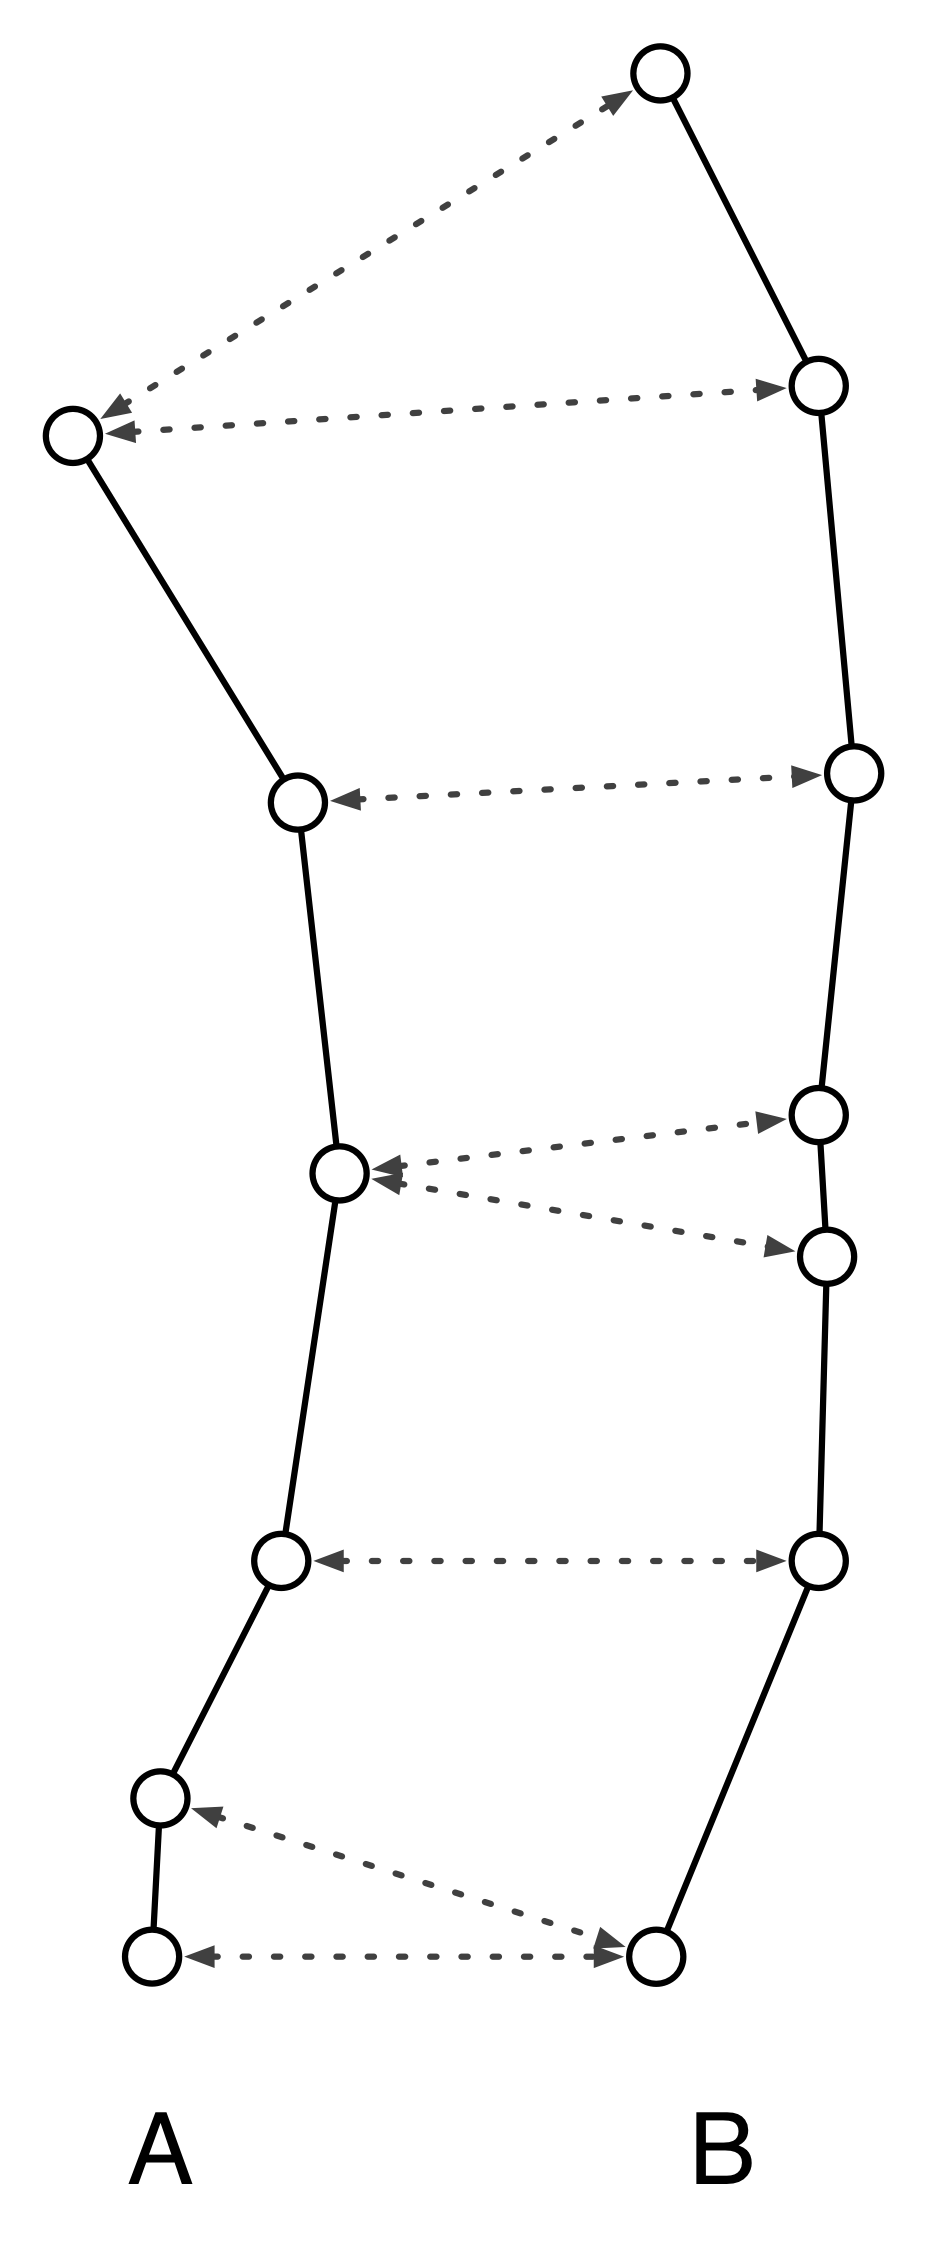
\includegraphics[width=4cm]{figures/dtw.png}
  \caption{Elastische Zuordnung bei DTW}
  \label{fig:dtw}
\end{figure}

Das gesuchte Minimum kann mithilfe von Dynamischer Programmierung gefunden werden. Gegeben die Rekurrenz
\begin{equation}
  \label{eqn:dp}
  \gamma(i,j) =
  \begin{cases}
    \sum_{k=0}^j \delta(a_0, b_k) & i = 0 \\
    \sum_{k=0}^i \delta(a_k, b_0) & j = 0 \\
    \delta(a_i,~b_j) + \min\{~\gamma(i-1,j-1),~\gamma(i-1,j),~\gamma(i,j-1)~\} & \text{sonst}
  \end{cases}  
\end{equation}

dann ist
\begin{equation}
  \label{eqn:dpdtw}
  DTW(A,B) = \frac{\gamma(n,m)}{K}
\end{equation}. \TODO Wo kommt das K her?

In dieser Form hat DTW die Laufzeit- und Speicherplatzkomplexität \(\mathcal{O}(nm)\). Darum wundert es nicht, dass bereits einige Wissenschaftler versucht haben, den Algorithmus zu optimieren. Auch für Detexify ist dieses Laufzeitverhalten nicht ausreichend um eine Erkennung in Echtzeit zu ermöglichen.


\subsection{Beschränkung des Warping-Pfads} % (fold)
\label{sub:constrained_warping_window}

\begin{figure}
  \centering 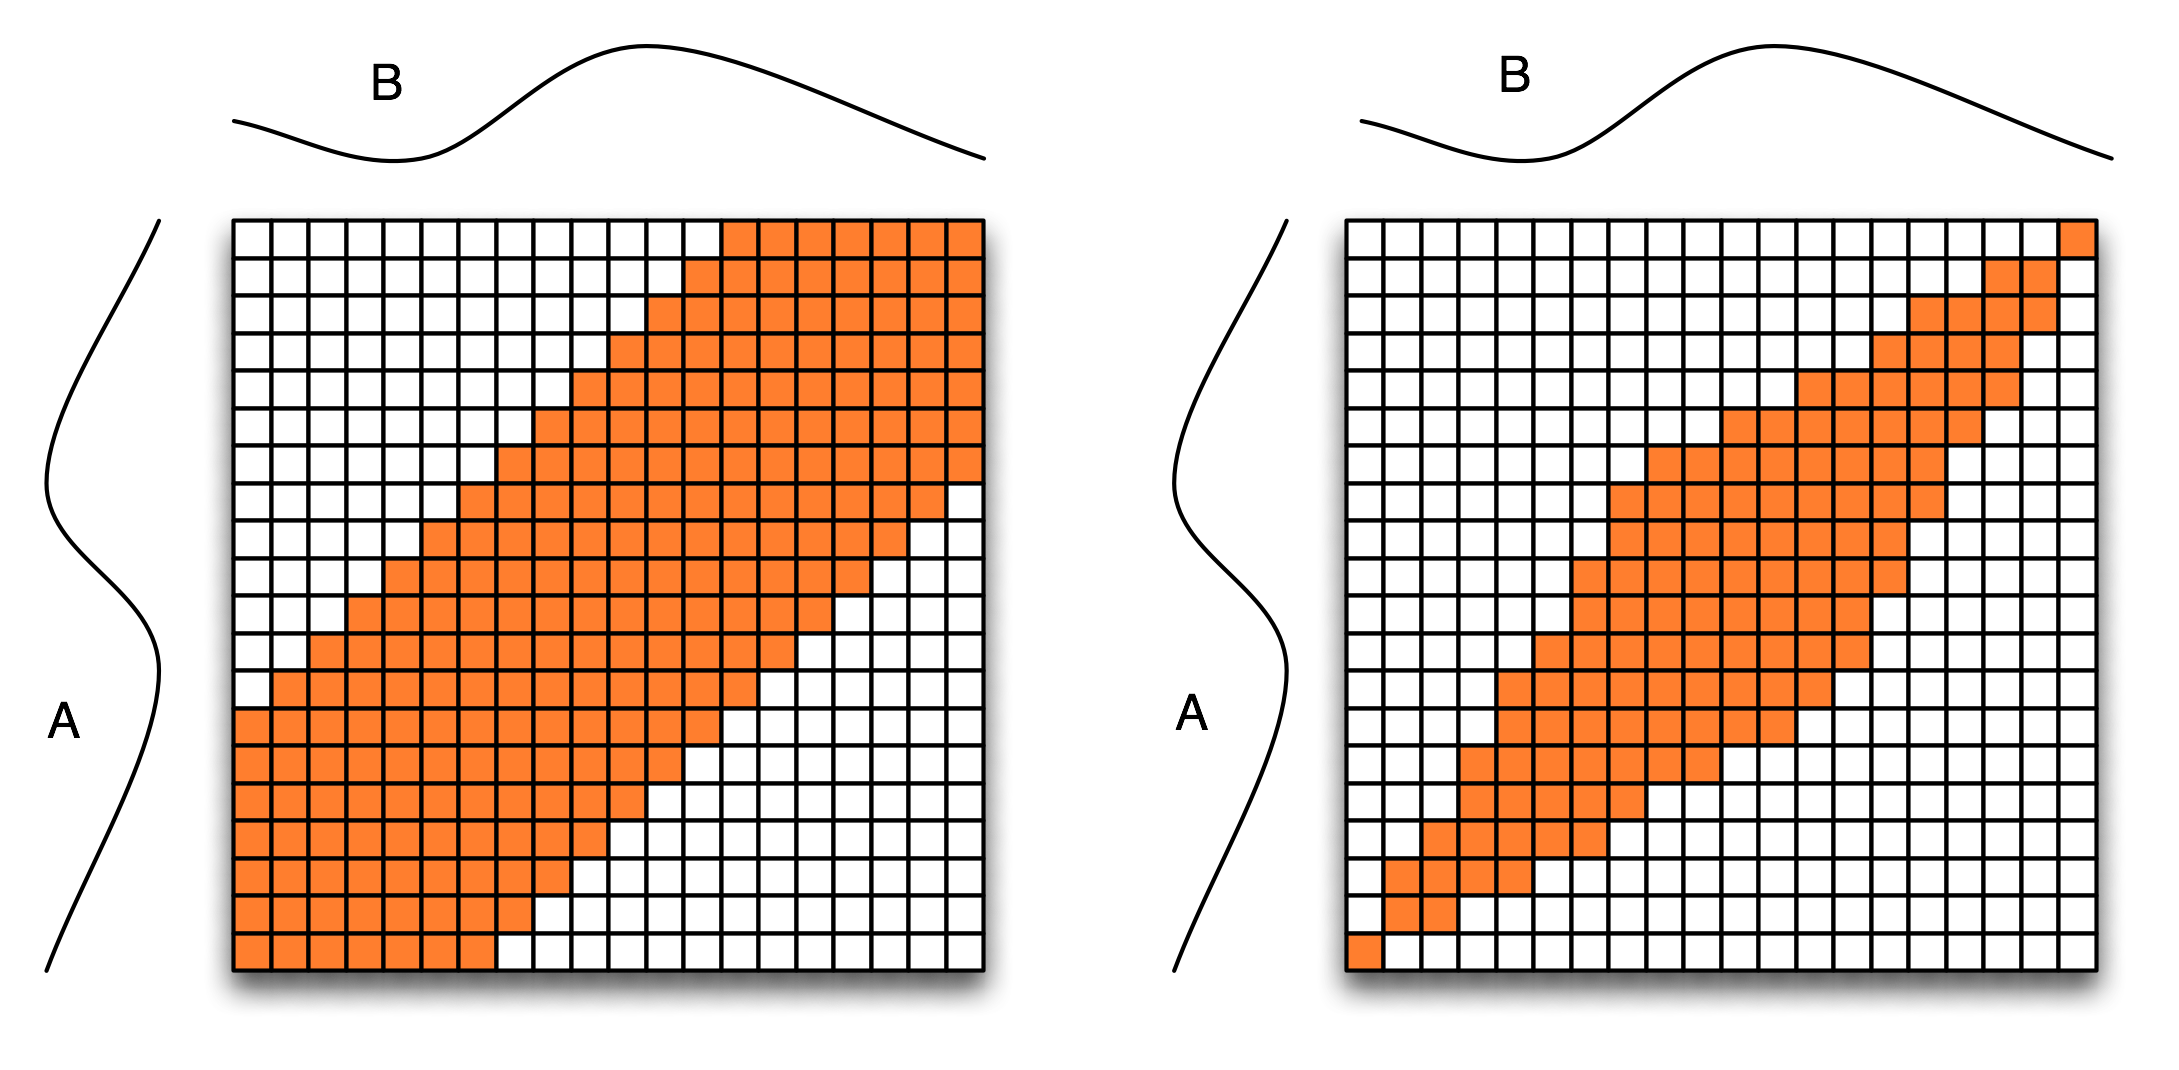
\includegraphics[width=\textwidth]{figures/constraints.png}
  \caption{Typische Beschränkungen das Warping-Pfades}
   Links: Sakoe-Chiba-Band, Rechts: Ikatura-Parallelogramm
  \label{fig:constraints}
\end{figure}


Es ist möglich DTW dadurch zu beschleunigen, dass bei der Suche nach dem optimalen Warping-Pfad nicht die ganze Matrix durchsucht wird. Stattdessen wird der Suchraum beschränkt. Abb.~\ref{fig:constraints} zeigt üblicherweise verwendete globale Beschränkungen. Es ist auch möglich lokale Beschränkungen wie in \cite{Rabiner:1993p11752} beschrieben festzulegen, \citet{Keogh:2005p7751} bemerken aber, dass das im Prinzip dasselbe, wie globale Beschränkungen sind, darum gehe ich darauf nicht näher ein. Nun könnte man glauben, dass sich eine solche Einschränkung nachteilig auswirkt. \citet{Ratanamahatana:2004p7522} berichten aber in ihrer Arbeit, dass eher das Gegenteil der Fall ist und Beschränkungen des Pfades sogar helfen, die Erkennungsraten zu verbessern. Dies kann dadurch verstanden werden, dass durch Beschränkungen pathologisches Warpen verhindert wird \cite{Keogh:2005p7751}.
%- Leichte Geschwindigkeitsverbesserung \( \mathcal{O}(ns) \) für fest gewähltes $s$
%- Sakoe and Chiba 1978 haben wohl schon rausgefunden, dass globale beschränkungen helfen \cite{Keogh:2005p7751}

Wenn beide Folgen die gleiche Länge $n$ haben, ist eine Möglichkeit den Warping-Pfad zu beschränken, einen Korridor um die Diagonale der Matrix festzulegen, aus dem nicht ausgebrochen werden darf. Beschrieben werden kann dies durch eine Beschränkung der Indizes des Warping-Pfades \( w_k = (i,j)_k \) und zwar gilt dann
\begin{equation}
  \label{eq:constraints}
  j−r(i) \leq i \leq j+r(i)
\end{equation}
, wobei $r(i)$ den erlaubten Korridor beschreibt.

Im Fall von \(r(i) = s\) also $r$ konstant reduziert sich damit die Komplexität von DTW von \( \mathcal{O}(n^2) \) auf \( \mathcal{O}(ns) \). Zusätzlich ermöglicht die Beschränkung aber eine weitere viel effektivere Optimierung:

\subsection{Untere Schranken} % (fold)
\label{sub:lower_bounding}

Gegeben ein Abstandsmaß \( \delta : S\times S \rightarrow \mathbb{R}_0^+ \) und eine untere Schranke \( \delta_{LB} \) d.h. \( \delta_{LB}(a,b) \leq \delta(a,b) ~\forall~ a,b \in S \), die deutlich günstiger zu berechnen ist, dann lässt sich mit dem folgenden naiven Algorithmus eine sequentielle Suche nach dem nächsten Nachbarn eines Elementes \( c \in S \) beschleunigen (vergl. \cite{Keogh:2005p7751}).

\begin{algorithm}
  \caption{Beschleunigung der Suche nach dem nächsten Nachbarn eines Elementes \(c\) durch eine untere Schranke}
  \begin{algorithmic}
    \STATE $\text{best\_so\_far} \gets \infty$
    \FORALL{samples $s$}
      \STATE $\text{lb\_dist} \gets \delta_{LB}(c,s)$
      \IF{$\text{lb} < \text{best\_so\_far}$}
        \STATE true\_dist $\gets \delta(c,s)$
        \IF{$\text{true\_dist} < \text{best\_so\_far}$}
          \STATE best\_so\_far $\gets$ true\_dist
          \STATE nearest\_neighbor $\gets s$
        \ENDIF
      \ENDIF
    \ENDFOR
  \end{algorithmic}
\end{algorithm}

Für DTW für Folgen derselben Länge $n$ mit reellen Messpunkten mit einer Beschränkung des Warping-Pfades der Form \ref{eq:constraints} haben \citet{Keogh:2005p7751} eine scharfe untere Schranke angegeben. Zudem haben \citet{Ratanamahatana:2004p7522} die Kritik entkräftet, dass vor der Verwendung einer solchen Optimierung eine lineare Interpolation der Folgen nötig ist, um sie auf dieselbe Länge zu bringen, und damit der Vorteil Folgen unterschiedlicher Länge vergleichen zu können verlogen ginge. Eine untere Schranke scheint also eine reizvolle Möglichkeit zu sein DTW zu beschleunigen.

\TODO wer hat vor \citet{Keogh:2005p7751} untere Schranken angegeben? Muss ich das erwähnen?

In Fall von Detexify sind die einzelnen Punkte der Folgen aber Punkte im \( \mathbb{R}^2 \) (siehe \ref{sec:vorverarbeitung}) und es ist intuitiv einzusehen, dass eine Reduktion auf eine Dimension einen zu hohen Informationsverlust nach sich ziehen würde. Es ist zwar möglich auf eine zu \cite{Keogh:2005p7751} analoge Weise eine untere Schranke zu definieren, und das werde ich als nächstes tun - es zeigt sich jedoch, dass diese untere Schranke keine vorteilhaften Laufzeiteigenschaften mehr hat. Darum wird auch der formale Beweis, dass es sich wirklich um eine untere Schranke handelt übergangen.

\subsection{Eine untere Schranke für DTW für Folgen im \( \mathbb{R}^2 \)}

Bevor ich meine untere Schranke erkläre, gebe ich noch eine kurze Erklärung der von \citet{Keogh:2005p7751} definierten unteren Schranke LB\_Keogh.

Seien
\begin{align}
  Q &= q_1 \dots q_n \\
  C &= c_1 \dots c_n
\end{align}
zwei Folgen gleicher Länge $n$. \( \mathcal{W}_r \) sei die Menge der durch \(r\) beschränkten Warping-Pfade (siehe \ref{eq:constraints}). DTW sei (leicht verändert) gegeben durch

\begin{equation}
  \label{eq:keoghdtw}
  DTW(Q,C) = \min_{W \in \mathcal{W}_r}{\sqrt{\sum_{i=1}^n d_{w_i}}}
\end{equation}


Lorem ipsum dolor sit amet, consectetur adipisicing elit, sed do eiusmod tempor incididunt ut labore et dolore magna aliqua. Ut enim ad minim veniam, quis nostrud exercitation ullamco laboris nisi ut aliquip ex ea commodo consequat. Duis aute irure dolor in reprehenderit in voluptate velit esse cillum dolore eu fugiat nulla pariatur. Excepteur sint occaecat cupidatat non proident, sunt in culpa qui officia deserunt mollit anim id est laborum.

% subsubsection lower_bounding (end)

\subsection{linear space and time} % (fold)
\label{sec:linear_space_and_time}
Lorem ipsum dolor sit amet, consectetur adipisicing elit, sed do eiusmod tempor incididunt ut labore et dolore magna aliqua. Ut enim ad minim veniam, quis nostrud exercitation ullamco laboris nisi ut aliquip ex ea commodo consequat. Duis aute irure dolor in reprehenderit in voluptate velit esse cillum dolore eu fugiat nulla pariatur. Excepteur sint occaecat cupidatat non proident, sunt in culpa qui officia deserunt mollit anim id est laborum.
% subsubsection linear_space_and_time (end)

\subsection{\TODO Parameter} % (fold)
\label{sec:todo_parameter}

% subsubsection todo_parameter (end)

\citet{Golubitsky:2009p1842} enthält ganz viele Statistiken zu Parametern für DTW (und Vergleich mit Funktionalapproximationsmaß)
\begin{itemize}
  \item k (Anzahl der Nachbarn)
  \item Anzahl der Punkte
\end{itemize}


% eigentlich egal: siehe \cite{Vuong:2010p10279} Natural Log, symbol recognition is implemented using a statistical approach based on Gaussian Density Estimation \dots siehe auch \cite{Vuong:2010p10279} \TODO Paper suchen

\cite{MacLean:2010p9970} DTW in linear time and constant space

\cite{Watt:2005p1816} schlägt pruning durch klassische features vor

- DTW kann schwer durch Elimination (Pruning) optimiert werden, da DTW keine Metrik ist ~> Voronoi-Trick geht nicht also keine exakte Lösung. Vielleicht trotzdem mal Greedy-Algorithmus nach Hart (siehe Jiang-Script) testen?

- DTW/Elastic matching/DP matching wird benutzt für Lateinische Schriftzeihen, Chinesisch, \cite{Tappert:1990p10302}

weitere Argumente für KNN

-> gleicht Schreibstile aus wenn genug Muster
